\chapter{QEC decoders for color codes}
\label{chap:qec_decoders}

Having established the foundational principles of quantum error correction, and having explored both the structure and characteristics of color codes and the physical reality of error models, it is now time to address the final critical component of the QEC cycle: the decoders. A decoder is the classical algorithm responsible for transforming a set of syndrome measurements into a concrete diagnosis. In other words, it formulates a prediction of the error that has affected the logical observable, or equivalently, it infers the correct logical observable given the faulty measured one. The execution speed and accuracy of the decoders are major bottlenecks in realizing large-scale fault-tolerant quantum computation, and there's often a trade-off between them. Speed is relevant because the decoding process must ideally keep pace with the quantum circuit operation, as sometimes errors must be corrected during the execution. However, to increase decoding speed, accuracy may be sacrificed. 

\notatfm{The \textit{Decoder Error Model} is often referred to by different names in the literature: \textit{Syndrome Graph}, \textit{Decoding Graph} or \textit{Matching Graph}. Because our focus is in QEC simulation, we will prefer the term \textit{\textbf{Detector Error Model}} or DEM, which is the term used by \texttt{stim}. The DEM acts as a bridge between the physical noise phenomena (such as gate infidelities or readout errors) and the abstract graph or hypergraph structures used by most decoding algorithms to find the optimal correction.} To achieve high accuracy, a decoder must do more than just find any arbitrary error string that satisfies the observed syndrome; it must ideally identify the most probable error chain. At this point, we must introduce the concept of the \textit{Decoding Graph} or \textbf{Detector Error Model}, DEM. The DEM is a structured representation that captures the specific probabilities of the different error mechanisms that trigger detection events in the quantum circuit. By incorporating a DEM, decoders can leverage these probability distributions to make informed decisions. This additional statistical context allows the decoder to determine the actual error chain with a significantly higher success rate.

In this chapter, we will not dive into the programming aspects or the specific implementation details of decoders. The practical implementation of a basic decoder will be thoroughly covered in Chapter \ref{chap:implementation_and_simulation}, where it will also be compared against the standard Minimum Weight Perfect Matching (MWPM) algorithm to explicitly demonstrate the clear advantage of incorporating the DEM into the decoding process.


\section{Minimum Weight Perfect Matching (MWPM)}
\label{sec:mwpm}

\notatfm{MWPM relies in two fundamental things: \textbf{Perfect Matching}, meaning that it matches pairs of nodes with a set of edges, so no node is left unpaired and no node belongs to multiple matches, and \textbf{Minimum Weight}, meaning that the total weight of the selected set of edges is the minimum possible to perfectly match the active nodes.} The Minimum Weight Perfect Matching (MWPM) was the first algorithm to demonstrate that topological codes could be practically decoded. Its theoretical mapping to the surface code was established by Dennis, Kitaev, Landahl, and Preskill in 2002 \cite{dennis2002topological}. MWPM is arguably the most famous and widely used decoder in the field of quantum error correction. Originally conceived as a solution to a classical optimization problem by Jack Edmonds in 1965 \cite{edmonds1965paths}, MWPM is designed to find a perfect matching in a weighted graph such that the sum of the weights of the edges in the matching is minimized. 

In the context of QEC, and specifically for the Surface Code, the decoding problem maps naturally to a standard graph problem. When a single Pauli error occurs on a data qubit in a surface code, it typically flips the measurement outcome of exactly two adjacent stabilizers. These two activated stabilizers are the "defects" or "detection events" that form the syndrome. The decoding process consists of constructing a \textbf{syndrome graph} where:
\begin{itemize}
    \item \textbf{Nodes} represent the activated stabilizers.
    \item \textbf{Edges} represent the possible physical errors (or chains of errors) that could have caused those stabilizers to flip.
    \item \textbf{Weights} on the edges are assigned based on the error probabilities. Lower probability errors are assigned higher weights.
\end{itemize}




\begin{figure}[hbt!]
    \centering
    % SUBFIGURE A: PHYSICAL LATTICE
    \begin{subfigure}[b]{0.45\textwidth}
        \centering
        \resizebox{\linewidth}{!}{
        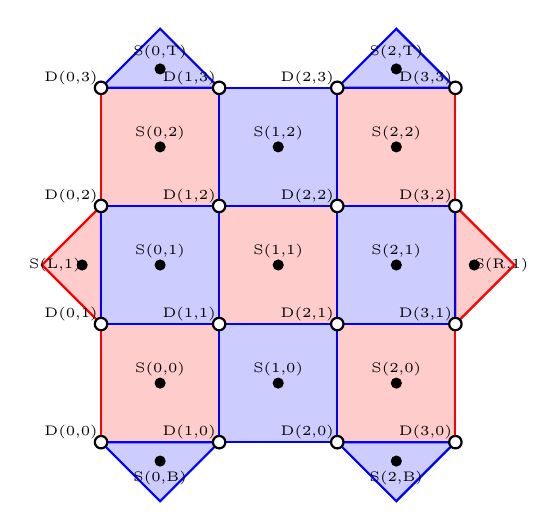
\begin{tikzpicture}[scale=1.5]
            % Z-stabilizers (Red full faces)
            \foreach \x/\y in {0/0, 2/0, 1/1, 0/2, 2/2} {
                \filldraw[red!20, draw=red, thick] (\x,\y) rectangle (\x+1, \y+1);
                \node[font=\tiny, inner sep=0.5pt] at (\x+0.5, \y+0.62) {S(\x,\y)};
            }
            
            % Z-stabilizers (Red half faces - Rough boundaries)
            \filldraw[red!20, draw=red, thick] (0,1) -- (0,2) -- (-0.5, 1.5) -- cycle; 
            \node[font=\tiny, inner sep=0.5pt] at (-0.39, 1.5) {S(L,1)};
            
            \filldraw[red!20, draw=red, thick] (3,1) -- (3,2) -- (3.5, 1.5) -- cycle; 
            \node[font=\tiny, inner sep=0.5pt] at (3.39, 1.5) {S(R,1)};
        
            % X-stabilizers (Blue full faces)
            \foreach \x/\y in {1/0, 0/1, 2/1, 1/2} {
                \filldraw[blue!20, draw=blue, thick] (\x,\y) rectangle (\x+1, \y+1);
                \node[font=\tiny, inner sep=0.5pt] at (\x+0.5, \y+0.62) {S(\x,\y)};
            }
            
            % X-stabilizers (Blue half faces - Smooth boundaries)
            \foreach \x in {0, 2} {
                \filldraw[blue!20, draw=blue, thick] (\x,0) -- (\x+1,0) -- (\x+0.5, -0.5) -- cycle;
                \node[font=\tiny, inner sep=0.5pt] at (\x+0.5, -0.3) {S(\x,B)};
                
                \filldraw[blue!20, draw=blue, thick] (\x,3) -- (\x+1,3) -- (\x+0.5, 3.5) -- cycle;
                \node[font=\tiny, inner sep=0.5pt] at (\x+0.5, 3.3) {S(\x,T)};
            }
        
            % Ancilla Qubits (Solid black dots, reduced size)
            \foreach \x/\y in {0.5/0.5, 2.5/0.5, 1.5/1.5, 0.5/2.5, 2.5/2.5, 1.5/0.5, 0.5/1.5, 2.5/1.5, 1.5/2.5} {
                \filldraw[black] (\x,\y) circle (1.2pt);
            }
            \filldraw[black] (-0.16, 1.5) circle (1.2pt);
            \filldraw[black] (3.16, 1.5) circle (1.2pt);
            \foreach \x in {0.5, 2.5} {
                \filldraw[black] (\x, -0.16) circle (1.2pt);
                \filldraw[black] (\x, 3.16) circle (1.2pt);
            }
        
            % Data Qubits (White circles, reduced size)
            \foreach \x in {0, 1, 2, 3} {
                \foreach \y in {0, 1, 2, 3} {
                    \filldraw[black, fill=white, thick] (\x,\y) circle (1.5pt);
                    \node[above left, font=\tiny, inner sep=1pt] at (\x,\y) {D(\x,\y)};
                }
            }
            
        \end{tikzpicture}
        }
        \caption{}
        \label{fig:mwpm_lattice}
    \end{subfigure}
    \hfill
    % SUBFIGURE B: SYNDROME GRAPH
    \begin{subfigure}[b]{0.45\textwidth}
        \centering
        \resizebox{\linewidth}{!}{
        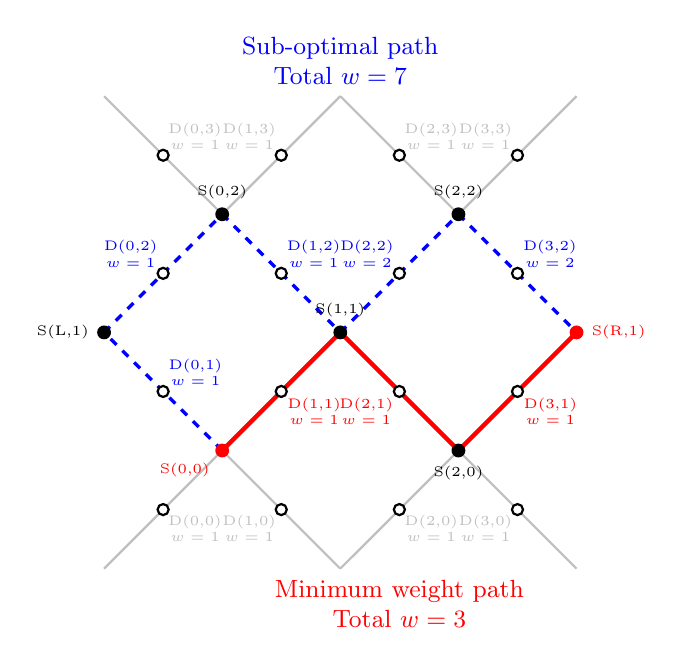
\begin{tikzpicture}[scale=1.5]
            % Styles matching the new sizing and background removal
            \tikzset{
                syndrome/.style={circle, fill=black, inner sep=0pt, minimum size=5pt},
                defect/.style={circle, fill=red, inner sep=0pt, minimum size=5pt},
                edge/.style={gray!50, thick},
                edge_marker/.style={circle, draw=black, fill=white, thick, inner sep=0pt, minimum size=4pt},
                lbl/.style={font=\tiny, align=center, inner sep=1.5pt}
            }
            
            % Perfect 45-degree mathematical coordinates
            \coordinate (C00) at (0.5, 0.5);
            \coordinate (C20) at (2.5, 0.5);
            \coordinate (C11) at (1.5, 1.5);
            \coordinate (C02) at (0.5, 2.5);
            \coordinate (C22) at (2.5, 2.5);
            \coordinate (CHL) at (-0.5, 1.5); % Aligned to logical grid
            \coordinate (CHR) at (3.5, 1.5);  % Aligned to logical grid

            % 8 Boundary edges terminating at the virtual boundaries
            \foreach \start/\dest/\dlabel/\pos in {
                C00/{-0.5, -0.5}/{D(0,0)}/below right,
                C00/{1.5, -0.5}/{D(1,0)}/below left,
                C20/{1.5, -0.5}/{D(2,0)}/below right,
                C20/{3.5, -0.5}/{D(3,0)}/below left,
                C02/{-0.5, 3.5}/{D(0,3)}/above right,
                C02/{1.5, 3.5}/{D(1,3)}/above left,
                C22/{1.5, 3.5}/{D(2,3)}/above right,
                C22/{3.5, 3.5}/{D(3,3)}/above left%
            } {
                \draw[edge] (\start) -- (\dest) node[midway, edge_marker] {} node[midway, \pos, lbl] {\dlabel\\$w=1$};
            }

            % Path 2 (Sub-optimal, blue dashed)
            \foreach \start/\dest/\dlabel/\weight/\pos in {
                C00/CHL/{D(0,1)}/1/above right,
                CHL/C02/{D(0,2)}/1/above left,
                C02/C11/{D(1,2)}/1/above right,
                C11/C22/{D(2,2)}/2/above left,
                C22/CHR/{D(3,2)}/2/above right%
            } {
                \draw[blue, dashed, very thick] (\start) -- (\dest) node[midway, solid, edge_marker] {} node[midway, \pos, lbl, text=blue] {\dlabel\\$w=\weight$};
            }

            % Path 1 (Optimal, red solid)
            \foreach \start/\dest/\dlabel/\weight/\pos in {
                C00/C11/{D(1,1)}/1/below right,
                C11/C20/{D(2,1)}/1/below left,
                C20/CHR/{D(3,1)}/1/below right%
            } {
                \draw[red, ultra thick] (\start) -- (\dest) node[midway, edge_marker] {} node[midway, \pos, lbl, text=red] {\dlabel\\$w=\weight$};
            }

            % Place the 7 graph nodes covering the ends of the lines
            \node[syndrome] at (C20) {}; \node[below=2pt, font=\tiny] at (C20) {S(2,0)};
            \node[syndrome] at (C11) {}; \node[above=2pt, font=\tiny] at (C11) {S(1,1)};
            \node[syndrome] at (C02) {}; \node[above=2pt, font=\tiny] at (C02) {S(0,2)};
            \node[syndrome] at (C22) {}; \node[above=2pt, font=\tiny] at (C22) {S(2,2)};
            \node[syndrome] at (CHL) {}; \node[left=2pt, font=\tiny] at (CHL) {S(L,1)};
            
            % Highlight the active defects in red
            \node[defect] at (C00) {}; \node[below left=1pt, font=\tiny, text=red] at (C00) {S(0,0)};
            \node[defect] at (CHR) {}; \node[right=2pt, font=\tiny, text=red] at (CHR) {S(R,1)};

            % Display total path weights
            \node[blue, font=\small, align=center] at (1.5, 3.8) {Sub-optimal path\\Total $w=7$};
            \node[red, font=\small, align=center] at (2.0, -0.8) {Minimum weight path\\Total $w=3$};
            
        \end{tikzpicture}
        }
        \caption{}
        \label{fig:mwpm_graph}
    \end{subfigure}
    
    \caption{A visual representation of the Minimum Weight Perfect Matching problem under a code-capacity noise model. \textbf{(a)} The rotated surface code lattice introduced in Chapter~\ref{chap:state_of_the_art}. Data qubits are labeled as $D(x,y)$ and ancillas (stabilizers) as $S(x,y)$. \textbf{(b)} The full syndrome matching graph specifically for X-type errors, consisting of 7 nodes (the Z-stabilizer ancillas, shown as small black circles) and 16 edges (one for each physical data qubit--each possible X-type error in the code-capacity model--, represented by white circles indicating the weight (likeliness) of this error. Two possible error chains are highlighted, one of them being the one with minimum weight.}
    \label{fig:4:mwpm_example}
\end{figure}

The MWPM algorithm efficiently searches this graph to find the pairings of defects that minimize the total weight. This is illustrated in Figure \ref{fig:mwpm_graph}. Once the optimal pairing is found, the decoder identifies the most probable error chain and applies the corresponding correction. This approach is highly effective and its implementation (\cite{higgott2022pymatching}) serves as the benchmark against which almost all new decoders are measured.

\subsection{Edmonds' Blossom algorithm}
To understand how MWPM achieves this globally optimal pairing, it is necessary to look at its underlying mathematical engine: Edmonds' Blossom algorithm. A naive greedy approach—simply pairing the closest defects as soon as they are found—can easily get trapped in local minima, leaving isolated defects that force very high-weight connections later. Edmonds' algorithm systematically explores the graph to guarantee the absolute minimum weight solution.

This exploration is intuitively visualized using expanding regions. The algorithm begins by simultaneously growing a "bubble" outwards from every active defect. These bubbles expand across the adjacent data qubits in the graph, to other non-active defects. When the boundaries of two expanding bubbles collide, the two defects are temporarily matched. The algorithm assumes that the path followed by the bubbles corresponds to the chain of physical errors that connected them.

\notatfm{Let's see an example. Defects $A$ and $B$ are matched ($A \Rightarrow B$) and then defect $C$'s expanding bubble reaches $B$.  The path between them is stored as a non-matched path ($C \rightarrow B$). Defect $A$ is re-activated and it's bubble begins growing again. If the bubble reaches an active unmatched defect $D$, then an alternating path forms ($D \rightarrow A \Rightarrow B \rightarrow C$). This path has two non-matched segments and one matched segment. The algorithm "flips" the entire path's status ($D \Rightarrow A \rightarrow B \Rightarrow C$), correcting past suboptimal assumptions and increasing the total number of matched pairs.}As the bubbles continue to grow, they often encounter defects that are already matched to someone else, creating topological conflicts. The algorithm efficiently resolves these conflicts by re-evaluating its temporary matchings as new connections are discovered. Conflicting matches are resolved using \textit{alternating paths}—routes that alternate between currently assumed errors (matched edges) and assumed healthy qubits (unmatched edges). If an alternating path is found connecting two free defects, the algorithm "flips" the entire path's status, simultaneously correcting past suboptimal assumptions and increasing the total number of matched pairs.

Edmonds' algorithm succeeds where other algorithms fail because of how it handles cycling paths: the temporary connections form a closed loop consisting of an odd number of nodes. Odd-length cycles can't be paired internally (the flip will not fix the alternating chain). The Blossom algorithm overcomes this by temporarily collapsing the entire odd-cycle into a single "super-node" or \textit{blossom}. This new blossom then resumes expanding as a single entity to find an external pair. Once all defects in the graph are paired, the algorithm unfolds the blossoms back into their original nodes and resolves the internal pairings. This continuous process of growing bubbles, shrinking odd-cycles, and unfolding them guarantees finding the most probable physical error chain.

\subsubsection*{The Challenge of MWPM in Color Codes}

While MWPM is exceptionally well-suited for Surface Codes, it cannot be directly applied to 2D Color Codes. The reason lies in the fundamental topology of the code.

In a surface code, a physical error creates a 1-dimensional string connecting two defects. However, in a color code, a single physical Pauli error activates \textbf{three} adjacent stabilizers. Consequently, an error chain in a color code is not a simple path between two points, but a branching, 2-dimensional structure that connects multiple groups of three defects.

In the following sections we will study different alternatives to decode color codes, some of which heavily rely on MWPM.

\section{Union-find}

\label{sec:union_find}
\notatfm{The overall worst-case complexity is bounded by $O(V \alpha(V))$, where $V$ is the number of vertices and $\alpha(V)$ is the inverse Ackermann function—a function that grows so slowly that it evaluates to less than 5 for any practically conceivable graph size.} While the Minimum Weight Perfect Matching (MWPM) algorithm sets the standard for decoding accuracy, its worst-case computational complexity does not scale well with the number of nodes in the syndrome graph. Decoders must operate fast enough to prevent a backlog of uncorrected errors during the circuit execution, wich causes a bottleneck as fault-tolerant architectures scale to thousands of physical qubits. To address this speed bottleneck, Delfosse and Nickerson introduced the Union-find decoder in 2018 \cite{Delfosse_2021}, achieving an almost-linear worst-case complexity while maintaining a decoding threshold highly comparable to MWPM.
The primary innovation of the Union-find decoder is the replacement of the global path optimization of Edmonds' Blossom algorithm with a greedy solution. As said earlier, a naive greedy solution would easily fall into local minima. However, Union-find proposes a cluster-growth greedy strategy, similar to MWPM's one, but where, when two bubbles collide, they are merged and continue growing as long as they do not have a pair number of defects. When all clusters have a pair number of defects (which implies that all defects belong to a cluster), the second phase of the algorithm acts within each cluster to couple specific defects. The algorithm operates in two main sequential phases:
\begin{enumerate}
    \item \notatfm{The \textbf{Disjoint-Set} data structure tracks elements partitioned into disjoint subsets, supporting two efficient operations: \textbf{Find} identifies the root of a subset (the unique element of the subset that identifies this subset), and \textbf{Union} merges two subsets. Checking or merging clusters is executed in practically constant time, bringing the computational cost of the algorithm to near-linear with respect to the number of nodes.} \textbf{Cluster Growth:} Initially, every individual defect is placed in its own separate cluster. Using the standard \textit{Disjoint-Set} (or Union-find) data structure, the algorithm tracks these disjoint clusters. A cluster is classified as \textit{valid} if it contains an even number of defects, or if it touches a boundary. If a cluster is valid, its growth pauses. Conversely, any \textit{invalid} (odd-parity) cluster grows uniformly by absorbing its neighboring edges. When two growing clusters collide, the algorithm executes a \texttt{union} operation to merge them into a single, larger cluster. This iterative growth and merging process continues until every cluster in the graph becomes valid. As opposed to MWPM's blossom contraction, the Disjoint-Set data structure allows an easier handling of a cluster colliding with itself (creating an internal loop) thanks to the \textit{find} operator.
    
    \item \notatfm{At an intersection, if both (or neither) of the child branches bring an unpaired defect, the error strings are combined and the upwards node is left unmarked. If only one of the two branches brings an unpaired defect, then the upwards node is marked as an unpaired defect so the pruning can continue upwards.} \textbf{Path Resolution:} Once all clusters are validated, the algorithm must decide which specific edges inside each cluster correspond to the physical errors. For each valid cluster, the Union-Find process has already defined a tree (i.e. a graph without loops). This allows applying a highly efficient \textit{peeling algorithm}: starting from the leaf nodes of the tree and working toward the root, the algorithm greedily assigns error correction strings to pair all internal defects. From each leaf node, prunes are applied. If the node is a defect, the pruned edge is added to an error correction string and the next upwards node is marked as an unpaired defect to continue the pruning from it. When two branches intersect, the pruning on that path pauses until both branches reach the intersection point.
\end{enumerate}

The algorithm described so far does not account for different error probabilities. Because of that, it can lead to lower accuracy than MWPM. \textit{Weighted} variants of Union-find incorporate the DEM edge weights directly into the growth phase, causing clusters to grow faster through edges with higher probabilities (lower weights). This bridges the accuracy gap with MWPM while retaining fast execution speeds.

\subsubsection*{Application to Color Codes}
Like MWPM, the standard Union-find decoder is fundamentally a graph-based algorithm designed to pair defects connected by 1-dimensional strings. Consequently, applying Union-find directly to the branching hypergraphs of 2D Color Codes presents the exact same topological challenge outlined in Section~\ref{sec:mwpm}. To decode color codes efficiently, Union-find is typically integrated as the fast computational engine within reduction frameworks, such as Projection or Restriction decoders, which map the complex hypergraph onto standard surface code sub-graphs.

\section{BP+OSD}

\section{Projection decoders (Delfosse, 2014)}

\section{Restriction decoders (Kubica \& Delfosse, 2023)}

\section{Möbius decoder (Sahay \& Brown, PRX Quantum, 2022)}

\section{Concatenated MWPM decoder (Lee, Li \& Bartlett, Quantum, 2025)}

\section{Correlated matching decoder (Liu, Wu \& Lao, 2025)}
